%!TEX program = xelatex

\documentclass[11pt]{article}

\usepackage{hyperref}
\usepackage{graphicx}
\usepackage{wrapfig}
\usepackage{amssymb}
\usepackage{amsmath}
\usepackage{titlesec}
\usepackage{wrapfig}
\usepackage{caption}
\usepackage{subcaption}
\usepackage{sidecap}
\usepackage{clrscode}
\usepackage{xcolor}
\usepackage{float}
\usepackage{stackengine}

\usepackage[margin=0.75in]{geometry}

\newlength{\tindent}
\setlength{\tindent}{\parindent}
\setlength{\parindent}{0pt}
\renewcommand{\indent}{\hspace*{\tindent}}

\newcommand\tab[1][1cm]{\hspace*{#1}}
\newcommand{\SK}{\textbf{[SK]}\tab}
\newcommand{\KY}{\textbf{[KY]}\tab}
\newcommand{\CO}{\textbf{[CO]}\tab}
\newcommand\cdate[1][1cm]{\textbf{[#1]}}

\renewcommand{\thesubsection}{\thesection.\alph{subsection}}
\titleformat{\subsection}[runin]{\normalfont\large\bfseries}{\thesubsection}{1em}{}

\begin{document}

\begin{centering}
\Large
    \textbf{Bayesian Clustering and Topic Modeling of Gene Expression Data}  \\
    \vspace{2mm}
    \normalsize
    Skanda Koppula (\url{skoppula@mit.edu}), Karren Yang (\url{karren@mit.edu}) \\
    \vspace{2mm}
    \normalsize
    6.882 Project Proposal, \today \\
\end{centering}
\vspace{5mm}

\section{Overview}

We explored the usage of various topic and clustering models in the analysis of gene expression data. For the former, we explored whether topic modeling could identify biologically relevant `topics'. In this context, a `topic' is a set of genes that together perform a specific biological function (a `gene module'); we compared our results to modules found by biology literate. For the latter, we explored whether we are able to cluster cells
accurately based on their gene expression levels. \footnote{The genes in gene modules generally move in tandem: so when a gene module is upregulated, all genes have higher expression (i.e. frequency). This motivates our use of topic models to capture this relationship.}.

\section{Topic Model: Latent Dirichlet Allocation}

We were unable to yield any results using Python's out-of-the-box implementation of \texttt{lda} \cite{lda}. With our 250 MB dataset, the collapsed Gibbs sampler used in the implementation was taking too long to produce samples, even on larger server-grade machines and with a small number of LDA clusters. We explored modifying the source to parallelize the sampling, but found the source to be crabbed and hard to follow. \\

In our search for an alternative, we explored another implementation that used online variational bayes for posterior estimate \cite{ovb, online}, and a broken \texttt{C++} Gibbs sampler for LDA that we modified to work \cite{plda}. We were able to get this latter sampler running parallel across multiple cores, with a burn-in of 100 iterations. We compare these two posterior estimation approaches using our entire dataset, with a 10\% held-out testing partition. We experimented with $k=5,10,25,\text{ and } 50$ clusters.

Figure \ref{fig:time} in the Appendix shows the time to complete each estimation method. As expected, Gibbs scales poorly with the parameter dimensionality and is strictly worse than online variational Bayes across all studied topic counts.

Figure \ref{fig:time} in the Appendix shows the time to complete each estimation method. As expected, Gibbs scales poorly with the parameter dimensionality and is strictly worse than online variational Bayes across all studied topic counts.

Note that these $p$-values do \textit{not} factor for multiple hypothesis corrections, so could be misleadingly significant.

\section{Division of Work}

\section{Remaining Work and Schedule}
- robust to dropout
- time series

\section{Appendix}
\begin{figure}
    \label{fig:time}
    \centering
    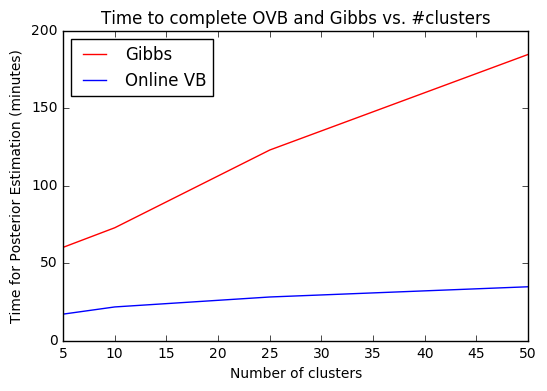
\includegraphics[width=0.5\textwidth]{time}
    \caption{Comparison of the running times of each of the posterior estimation methods across various cluster sizes.}
\end{figure}

\begin{figure}
    \label{fig:ll}
    \centering
    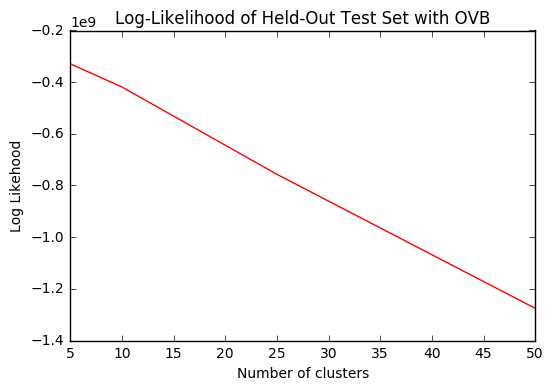
\includegraphics[width=0.5\textwidth]{ll}
    \caption{Log-likelihood of the held-out testing set, across various cluster sizes.}
\end{figure}

\begin{thebibliography}{9}
    \bibitem{nature} 
        The XL-mHG Test For Enrichment: A Technical Report.
        \url{https://arxiv.org/pdf/1507.07905.pdf}
         
    \bibitem{msigdb} 
        Molecular Signatures Database v6.0.
        \url{http://software.broadinstitute.org/gsea/msigdb}
         
    \bibitem{lda} 
        lda: Topic modeling with latent Dirichlet Allocation.
        \url{http://pythonhosted.org/lda/}

    \bibitem{ovb} 
        Online Latent Dirichlet Allocation with variational inference.
        \url{https://github.com/scikit-learn/scikit-learn/blob/master/sklearn/decomposition/online_lda.py}

    \bibitem{plda} 
        C++ implementation of Latent Dirichlet Allocation
        \url{https://github.com/openbigdatagroup/plda/blob/master/lda.cc}

    \bibitem{online}
        Online Learning for Latent Dirichlet Allocation.
        \url{https://pdfs.semanticscholar.org/157a/ef34d39c85d6576028f29df1ea4c6480a979.pdf}

    \bibitem{HDP}
        Hierarchical Dirichlet Processes
        \url{http://people.eecs.berkeley.edu/~jordan/papers/hdp.pdf}

    \bibitem{IBP}
        The IBP Compound Dirichlet Process and its Application to Focused Topic Modeling
        \url{http://www.cs.columbia.edu/~blei/papers/WilliamsonWangHellerBlei2010.pdf}

    \bibitem{TS-DDP}
        A Time-Series DDP for Functional Proteomics Profiles
        \url{https://www.ma.utexas.edu/users/pmueller/pap/NM12.pdf}


\end{thebibliography}


\end{document}
